
\graphicspath{ {mainmatter/Smallwood_2009/} }

\title*{2009: A History of Hemispherical Speakers at Princeton, Plus a DIY Guide}
\titlerunning{Hemispherical Speakers}


\author{Scott Smallwood, Perry Cook, Dan Trueman and Lawrence McIntyre}
\authorrunning{Smallwood et al.}


%\institute{Scott Smallwood \at Princeton University \email{skot@princeton.edu}
%\and Perry Cook \at Princeton University, \email{prc@[pton]}
%\and Dan Trueman\at Princeton University, \email{dtrueman@[pton]}
%\and Lawrence McIntyre \at Princeton University, \email{mcintyre@[pton]}}
%
%
\maketitle

\abstract*{This paper gives a historical overview of the development of alternative sonic
display systems at Princeton University; in particular, the design, construction,
and use in live performance of a series of spherical and hemispherical speaker
systems.  We also provide a DIY guide to constructing the latest series of
loudspeakers that we are currently using in our research and music making.}

\section{Introduction}

In developing new instruments for musical expression, one of our main areas of
interest has been the end of the audio chain:  the loudspeaker. For several years
we have been investigating the use of alternative sonic display systems,
resulting in a number of novel spherical and hemispherical speakers.

As we have wrangled with the conventional means of amplification of electronic
sounds, particularly in situations in which we have attempted to merge our sonic
and musical concerns with acoustic musicians, there have been many serious issues
raised.  For example, one of the advantages of playing a conventional acoustic
instrument is the unspoken ability to work with the dimension of space and
location.  Imagine a small group of acoustic musicians playing together, such as
a string quartet or a jazz combo. As a player in this ensemble, the relationships
and interactions with other musicians are based not only on the kinds of sounds
that are created, but also on the specificity of the player's location in space
with respect to other players, and the implications that physical and present
musical being presents to the ensemble as a whole.

In the realm of electronic music, these basic issues become problematic, and
have for years given way to a different kind of relationship between electronic
and acoustic musicians.  For example, consider a typical computer music concert
in which an electronic performer's sound absorbs and dominates the sonic space
through the stereo sound field of a modern PA system, or further, through a
massive surround system of multiple loudspeakers.  In this environment, any
acoustic musician involved becomes overwhelmed by the sonic and spatial power of
this system, and is forced to submit to an artificially narrow sonic space, or is
simply absorbed into the mix by being amplified (or ``processed'') and thrust
into a dislocated sonic field.  This can result in some powerful performance
paradigms, but the subtleties of ensemble space and location are lost, as well as
a true distinction between the acoustic performer and the electronics (not to
mention the social implications of such an absorption).  This is not to say that
spatial concerns are not dealt with; they become a kind of ``outside-in''
approach, in which sounds are placed in the stereo field, or in the multi-channel
surround environment, necessitating a ``sweet spot'' that, unfortunately, the
performers themselves are rarely able to gain access to.

Much of our work over the past few years has been to both \textit{reduce} the
sonic power of electronic musicians and to increase the \textit{spatial}
abilities of those voices; not only in order to more effectively combine
electronic voices with acoustic ones, but to reclaim the powerful ensemble
relationships that inherently exist in purely acoustic ensembles.  In short, we
are interested in reducing the overwhelming dispersion and density of electronic
music in exchange for the subtly of chamber and orchestral traditions.  So a
laptop orchestra is much more than a gathering together of many laptop musicians;
it is about finding ways of working with many voices in space and time, and
creating an ensemble in which ensemble space and location are reclaimed as
important and individual sonic concepts.

The result of such concerns has taken us in many different directions, from
using guitar amps for amplification to performing with small, near-field
monitors.  The problems with these systems, of course, is that they are
front-firing systems that do not radiate out in all directions the way acoustic
instruments do, thus creating sonic imbalance both within the ensemble and even
in the audience (try sitting in the direct line of fire of a guitar amp).  Thus,
we have developed a series of spherical and hemispherical ``inside-out''
loudspeakers that attempt to replicate the behavior of acoustic instruments. 
Through many years of trial and error, and also of observing the excellent work
of others, including the Compact Spherical Loudspeaker Array developed at CNMAT
in Berkeley \cite{Avizienis:2006}, and the IRCAM digitally controlled 3D array of loudspeakers \cite{Warusfel:2004},
we have settled upon a hemispherical design that is lightweight, compact, and
compatible with any laptop.  This has been an important concern since, in
addition to the fact that we individually gig with our speakers on a regular
basis, we also have also been working with large groups of players via the
Princeton Laptop Orchestra (PLOrk) \cite{Trueman:2006}, which has necessitated a large number of
speakers (we can accommodate well over 25 players at this point).

What follows is a short history of our research, design, engineering, and
construction, as well as a description of our latest hemispherical speaker
design. In addition, we provide instructions for making your own self-amplified
hemispherical speaker.

\section{The Near Complete History of Princeton  Spherical and Hemispherical Speakers }

\subsection{1997}

It all began with Dan Trueman, and his dissatisfaction with using guitar
speakers to amplify his electric violin. Perry Cook took this to heart, and
paying a visit to Bed Bath \& Beyond and Radio Shack, he took up his trusty saber
saw and other tools. ``The Bomb'' resulted (Figure~\ref{Smallwood:img-1}a). Disturbed by the lack of
isolation of the individual speaker drivers, Perry paid a visit to many Radio
Shacks and a Home Depot. This resulted in ``The Boulder'' (Figure~\ref{Smallwood:img-1}b).

Being an IKEA type, Dan secured some wooden salad bowls (as opposed to the metal
ones used for the Bomb). After some time in the Cook basement speaker lab, the
spher-o-nauts had some seriously cracked bowls on their hands. The bowls had to
go to Long Island for ``glue and clamp rehab'' in the wood shop of Dr. Trueman
Sr. With some tom-tom mounts and legs, ``R2'' was born (Figure~\ref{Smallwood:img-1}c).

\subsection{1998}

Aside from his other talents, Dr. Laurence Trueman (Dan's dad) is one wicked
good woodworker. He worked out the angles for his power saw so it could cut hunks
of wood such that they assemble into a wonderful sphere with twelve individual
enclosures (think ``Best of Boulder and Bomb''). Alliterations nearly aside,
``The Critter'' was created. This was integrated into the Bowed Sensor Speaker
Array (BoSSA) (Figure~\ref{Smallwood:img-1}d) \cite{Trueman:1999}.

\begin{figure}[t]
\centering
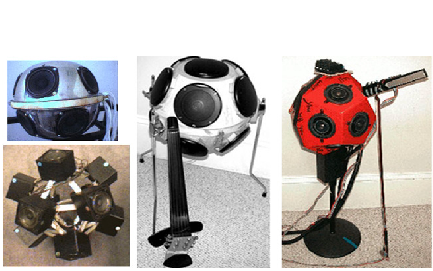
\includegraphics[width=\textwidth]{img-1-eps-converted-to-crop.pdf}
\caption{(a) Bomb. (b) Boulder. (c) R2. (d) BoSSA.}
\label{Smallwood:img-1} 
\end{figure}




\subsection{1999}

Growing weary of building spheres by hand, Dan and Curtis Bahn found United
Speaker Enclosures, who were selling spheres with one driver in them. We
convinced them to make us a bunch of spheres and hemispheres with 12 (and 6)
speaker mounting holes. ``Generation 2'' was born ((Figure~\ref{Smallwood:img-2}a). (Figure~\ref{Smallwood:img-2}b shows the
DigitalDoo, integrating an ancient instrument with sensors, mics, and a
hemispherical speaker.

Meanwhile, Bahn had become infected with the spherical speaker virus, and set
out to make a really big one based on the design of ``The Critter,'' for use with
his sensor bass. The result: ``Bubba'' (Figure~\ref{Smallwood:img-2}c) Once he had made the biggest,
Curtis wanted to make the smallest too, but to emphasize portability and sensor
control of sound and music performance. Out popped the ``Bubba Ball,'' (Figure~\ref{Smallwood:img-2}d)
which was not really a spherical speaker, but a controller heavily inspired by
one.  Soon it was common to see Dan, Curtis, Perry, and others playing together
with strange looking spherical and hemispherical speakers in a variety of live
performance situations \cite{Trueman:2000}.

\begin{figure}[t]
\centering
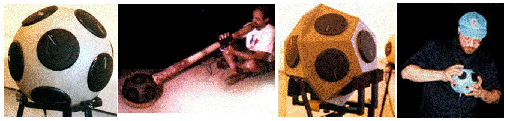
\includegraphics[width=\textwidth]{img-2-eps-converted-to-crop.pdf}
\caption{(a) Gen2. (b) DigitalDoo.  (c) Bubba.  (d) Bubba Ball.}
\label{Smallwood:img-2}
\end{figure}


\subsection{2001}

Stephan Moore, a graduate student working with Curtis Bahn at Rensselaer
Polytechnic Institute, worked with his professional cabinet maker uncle, Ken
Malz, to create lots and lots of these nice hemis of ``Generation 3'' (Figure~\ref{Smallwood:img-3}a).

\subsection{2005}

Dan Trueman, Perry Cook, Ge Wang, and Scott Smallwood started the Princeton
Laptop Orchestra (PLOrk) in the fall of 2005 \cite{Smallwood:2008,Trueman:2006,Trueman:2007,Wang:2008a}. Meanwhile, Stephan
Moore and Ken Malz began designing an improved speaker, with better wood (MDF
board) and larger drivers. Cook, Trueman, and Smallwood tacked onto this a
multi-channel interface capability. This six-channel ``4$^{th}$ Generation
Hemi,'' the Gray Hemi, hit the scene. This hemi was also the first to be produced
and sold commercially, and is still being sold by Electrotap
(www.electrotap.com). (Figure~\ref{Smallwood:img-3}b).

\begin{figure}[t]
\centering
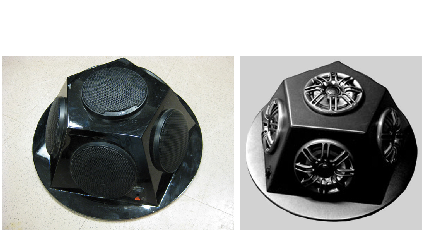
\includegraphics[width=\textwidth]{img-3-eps-converted-to-crop.pdf}
\caption{(a) Generation 3. (b) Generation 4.}
\label{Smallwood:img-3} 
\end{figure}



\subsection{2008: The Dawning of the Age of Delorean}
 Although the Gray Hemi design had provided years of success, one of the main obstacles for PLOrk was portability. Part of our weight and bulk issue had to do with amplification and interfacing. Since we have been using 6-channel hemispherical display systems, we require six channels of amplification per player, thus an external equipment rack populated with not only needed amplifiers (Stewart DA-70-2 and DA-70-4) but also the computer audio interfacing box (Edirol FA-101) as well as sensor/controller interfacing (Electrotap Tea-boxes).

Thanks to recent advances in amplifier technology, we began to explore integrating amplification electronics into the speaker enclosure. In addition, as interfacing technology has evolved, particularly in the areas of custom sensor interfacing and the widespread adoption of the USB 2.0 protocol for Human Interface Devices (HIDs), we were able to further eliminate the specialized devices that we had been using previously. The result is that we are now scaled down to two primary pieces of equipment: a laptop, and a hemispherical speaker containing its own amplification, with a small firewire audio interface mounted to the bottom of the speaker.  A third optional piece of equipment is a subwoofer, currently a Yamaha YST-FSW050. Figure~\ref{Smallwood:img-4-5}a shows our standard minimal PlorkStation for spring 2008.  Figure~\ref{Smallwood:img-4-5}b shows the newest ``Delorean'' speaker design.  Figure~\ref{Smallwood:img-4-5}c shows a  TeQWire Nano singer laptop/music stand with dual hemispherical speakers which are also self-amplified.


\begin{figure}[t]
\centering
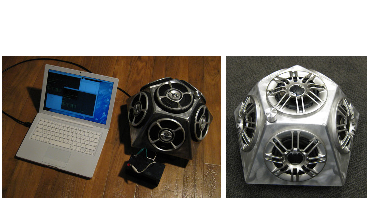
\includegraphics[height=42mm]{img-4-eps-converted-to-crop.pdf} 
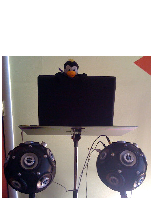
\includegraphics[height=42mm]{img-5-eps-converted-to-crop.pdf}
\caption{(a) PlorkStation '08 (b) Delorean (c) TeQWire Nano.}
\label{Smallwood:img-4-5}
\end{figure}



\section{Build Your Own Delorean}

The Delorean hemispherical speaker (Figure~\ref{Smallwood:img-4-5}b) is a self-amplified, six-channel
loudspeaker in an aluminum hemispherical case. It features a six-gang volume pot
that controls the overall volume of all six drivers.  The speaker requires a 4
Amp 12-Volt DC power source, and features a single 6-pin XLR jack to input six
line-level signals into the amps (requiring a special adapter).  The design is
also equipped to accommodate the mounting of a multiple-channel USB interface
underneath the speaker.  Here is a guide to constructing a Delorean and adapter
cables.

\subsection{Ingredients}

Two of the components for this project include custom designs: the
Charlize.\footnote{Charlize amp boards are available from DIY Paradise and Calv
Acoustic Labs at \url{http://diyparadise.com/w/charlize-744/} Our version includes DC
blocking capacitors, which also roll off frequencies below 80 Hz (we use subs for
the low end). There are also other manufacturers using the Tripath class-D amps
(T-amp).  We use the TA2020 at 10-20Watts (8$\Omega{}$-4$\Omega{}$) per channel.}
Amplifiers and the 6-gang potentiometers.\footnote{The potentiometer was custom
built by potentiometers.com  according to our specifications: Series 70,
conductive plastic, 3/4" shaft with 3/8" bushing and 3/8" shaft protruding. 50K
log taper, 6 gang.  As of January 2009, the part number is L26190.}  All other
parts are generally available from many electronics supply companies; obviously
you can substitute your own favorite speakers, knobs, etc.\footnote{For more
information about the specific parts we used, including a detailed parts list
with prices as of 2009, see
\url{http://silvertone.princeton.edu/~skot/plork/delorean/}.}

\subsection{Building the Speaker}

\subsubsection{Step 1: Building the Aluminum Shell}

Building this speaker first involves creating the shell. There are many
different ways to build a speaker shell. The one we describe here involves
cutting sheets of aluminum and welding them together, so it may not be for the
faint of heart. However, if suitable metal-shop skills and equipment are
available, these instructions will get you there. Ours were laid out and built by
Lawrence McIntyre in the Princeton University School of Engineering and Applied
Science Machine Shop (Figures~\ref{Smallwood:img-4-5}--\ref{Smallwood:img-7}).

\begin{description}
	\item[1a.] Cut out main body, cut large holes in all panels and half holes in half
panels. Drill and tap 8/32 holes in all panels excluding the half panels for
speaker mounts.

	\item[1b.] Bend up all panels 110 degrees. Weld at half panel joint. Sand joint
smooth.

	\item[1c.] Cut out, drill and tap bottom plate. Weld to main body. Sanding is not
necessary on the bottom plate.

	\item[1d.] Cut out top plate. Cut out large holes and drill and tap 8/32 holes for
speaker mounts. Weld to main body. Sand smooth with radius.

	\item[1e.] Fabricate jig to drill and tap 8/32 holes in half panels.

	\item[1f.] Apply finish
\end{description}


There are obviously other options available for creating shells. Our TeQWire nanos (Figure~\ref{Smallwood:img-4-5}c) are built using mixing bowls.  The Standford Laptop Orchestra uses hemispheres made from wooden salad bowls.  See also the Low Cost Spherical Speaker Array.\footnote{\url{http://www.instructables.com/id/Low-cost-Spherical-Speaker-Array}}

\subsubsection{Step 2: The Guts}

Once you have built the shell, it's time to build and mount the guts, which
includes the amplifiers, jacks, and volume pot, and all of the wiring to connect
everything together.  Standard 22 AWG stranded hookup wire works fine for all
wiring.

\begin{description}
	\item[2a.] Solder a common 12-inch ground wire to all the potentiometer grounding
terminals. (see Figure~\ref{Smallwood:img-8}).
	\item[2b.] Solder six 36-inch long colored wires to each of the pot's lower terminals,
and one 36-inch long black wire to the ground. Twist them together into a cable
harness.
	\item[2c.] Now solder six 8-inch long wires, using the same color scheme as the cable
harness above, to the middle, right-most terminal of each pot position. Twist
these together into three pairs, as shown:
	\item[2d.] Solder three pairs of the wires above to three different Charlize boards.
Whatever you chose for channels 1 and 2, for example, white-purple/purple, will
be soldered to the left and right input terminals of a Charlize board. Do the
same for channel pair 3 and 4, and pair 5 and 6.
	\item[2e.] Using red and black wire, solder the power terminals of each Charlize board
together and connect them to the coax jack; and include the ground common ground
wire of the pot in this power ground.
	\item[2f.] On each Charlize, solder an 8-inch pair of wires to the left and right
output terminals of the board. Use the same color scheme to identify channels.
For example, the white-purple/purple input wires of channels 1 and 2 match
white-purple/black for left out, and purple/black for right out.

\end{description}

\begin{figure}[t]
\centering
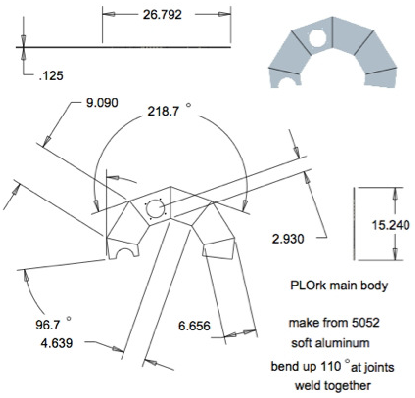
\includegraphics[width=\textwidth]{img-6-eps-converted-to-crop.pdf}
\caption{Main body of enclosure}
\label{Smallwood:img-6}
\end{figure}

\begin{figure}[t]
\centering
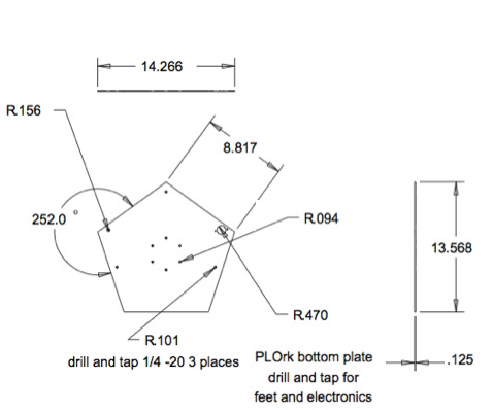
\includegraphics[width=85mm]{img-7-eps-converted-to-crop.pdf}
\caption{Bottom plate of enclosure}
\label{Smallwood:img-7}
\end{figure}

\begin{figure}[t]
\centering
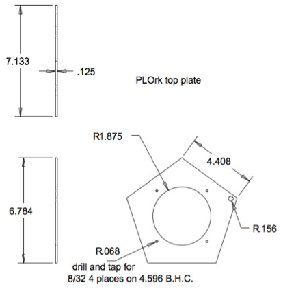
\includegraphics[width=70mm]{img-8-eps-converted-to-crop.pdf}
\caption{Top plate of enclosure}
\label{Smallwood:img-8}
\end{figure}

\begin{figure}[t]
\centering
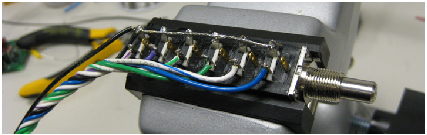
\includegraphics[width=\textwidth]{img-9-eps-converted-to-crop.pdf}
\caption{Input wiring of pot}
\label{Smallwood:img-9}
\end{figure}

\begin{figure}[t]
\centering
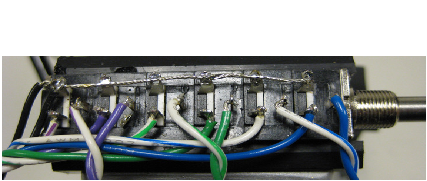
\includegraphics[width=\textwidth]{img-10-eps-converted-to-crop.pdf}
\caption{Output wiring of pot}
\label{Smallwood:img-10}
\end{figure}


\begin{figure}[t]
\centering
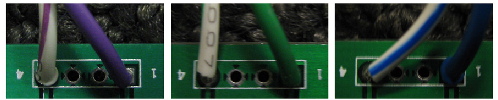
\includegraphics[width=\textwidth]{img-11-eps-converted-to-crop.pdf}
\caption{Input wiring to Charlize boards}
\label{Smallwood:img-11}
\end{figure}


\begin{figure}[t]
\centering
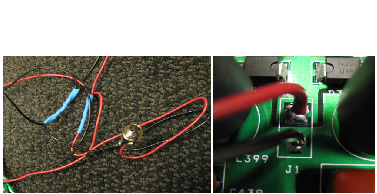
\includegraphics[width=\textwidth]{img-12-eps-converted-to-crop.pdf}
\caption{Power wiring}
\label{Smallwood:img-12}
\end{figure}


\begin{figure}[t]
\centering
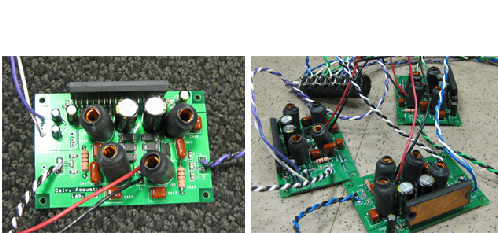
\includegraphics[width=\textwidth]{img-13-eps-converted-to-crop.pdf}
\caption{(a) Charlize board with all leads. (b) all three.}
\label{Smallwood:img-13}
\end{figure}

An important final step before mounting the guts inside the shell is to TEST
each amp channel to make sure it works. Plug the amps into a 12V power supply and
run test leads to each input on the pot from a line audio source (CD, iPod, etc.)
and connect a speaker temporarily to the corresponding output. If all works, go
on to the next stage.

\subsubsection{Step 3: Install the Guts}

This is a delicate and often frustrating operation that involves mounting the
amps and all of their appendages into the center of the shell. Here it is very
important to make sure the shell has the proper holes drilled.

\begin{description}
	\item[3a.] Mount short pieces of foam on each end of the back of the Charlize boards.
Then use nylon cable ties to fasten the three Charlize boards together into the
shape of a triangle. Don't connect the final side yet.

	\item[3b.] Stuff the boards into the shell through one of the speaker holes, and
fasten the final side together to finish the triangle. Position it in the center.
Mount the volume pot on top and the power jack on the bottom in their predrilled
holes.

	\item[3d.] Paint the bottom of each of the TRIAD amp chip with thermal adhesive. Then
position the board cluster in the center of the inside of the hemi so that the
six circular holes on the bottom will line up with the half-moon indentations on
the TRIAD amp chip of each board, as shown. Use 6-32 machine screws and nuts, and
be careful not to over-tighten! Use threadlocker on the screws and nuts. NOTE:
Orient the three amps towards the speaker holes whose speakers they will power,
if possible.

	\item[3e.] Thread the long cable harness from the volume pot through the jack mounting
hole. Solder the leads to pins 1-6 for channels 1-6, and solder the ground lead
to the  jack grounding terminal. Mount the jack using 4-40 machine screws.
Remember to use threadlocker! NOTE: Make sure that the tab on the jack faces the
right edge of the speaker.
\end{description}

\begin{figure}[t]
\centering
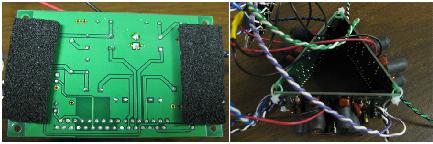
\includegraphics[width=\textwidth]{img-14-eps-converted-to-crop.pdf}
\caption{(a) Charlize foam mounting (b) 3-board cluster}
\label{Smallwood:img-14}
\end{figure}


\begin{figure}[t]
\centering
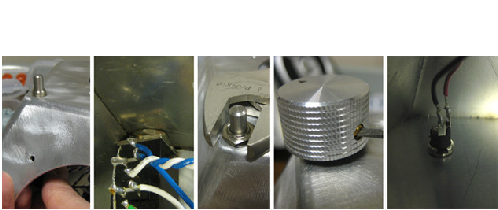
\includegraphics[width=\textwidth]{img-15-eps-converted-to-crop.pdf}
\caption{Potentiometer installation }
\label{Smallwood:img-15}
\end{figure}


\begin{figure}[t]
\centering
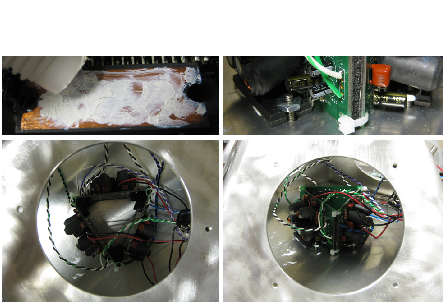
\includegraphics[width=\textwidth]{img-16-eps-converted-to-crop.pdf}
\caption{Mounting cluster inside speaker enclosure}
\label{Smallwood:img-16}
\end{figure}


\begin{figure}[t]
\centering
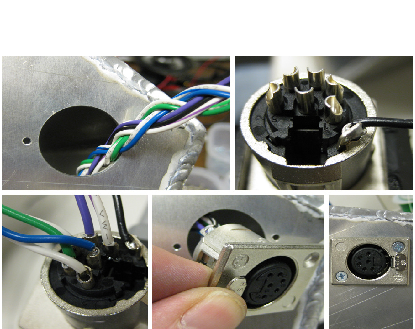
\includegraphics[width=\textwidth]{img-17-eps-converted-to-crop.pdf}
\caption{Audio input jack installation}
\label{Smallwood:img-17}
\end{figure}

\subsubsection{Step 4: Install the Speakers}

\begin{description}
	\item[4a.] Mount some foam around the openings for the speakers, enough so that any
flat metal or plastic part of the speaker flange will not rattle.
	\item[4b.] Pull out the appropriate pair of leads for each speaker, solder, and
carefully mount the speaker. Use threadlocker!
	\item[4c.] Before installing the sixth and last speaker (top), first fill the inside
of the speaker with acoustic fiber. Put in a lot of fiber---but don't over-stuff.
Make sure that wiring and boards are not pressed-upon too much.
\end{description}


\begin{figure}[t]
\centering
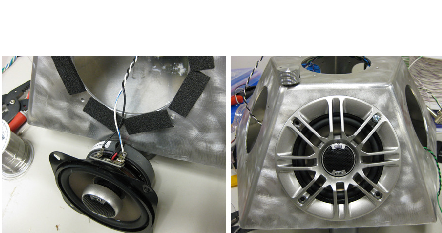
\includegraphics[width=\textwidth]{img-18-eps-converted-to-crop.pdf}
\caption{Solder, foam, and mount the speakers}
\label{Smallwood:img-18}
\end{figure}


\subsubsection{Testing}

Once the speakers are all in place, mounted, and ready to go, it's time to test
your speaker. This can be done in many ways, and should involve testing each
speaker independently and together with the others.

\begin{figure}[t]
\centering
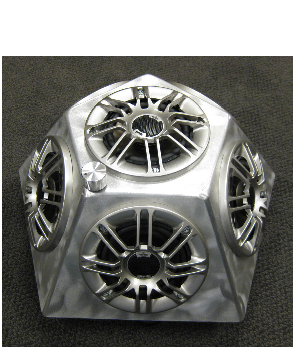
\includegraphics[width=70mm]{img-19-eps-converted-to-crop.pdf}
\caption{Completed Delorean.}
\label{Smallwood:img-19}
\end{figure}

\subsection{Connecting Cable/Adapters}

The audio inputs for the six channels are accomplished via a six-pin XLR jack.
You can build your own adapter, or you can order them custom from HAVE, Inc (they
will create custom cables for a fee---and they have made many of these for us). 
The adapter we use features an XLR male plug on one end, and six RCA male plugs
on the other.

Figure~\ref{Smallwood:img-20}a shows a six channel cable (we use this to connect to a U46 USB
interface, which is mounted under the speaker).  The tip from each RCA (or 1/4")
plug should be connected to one of the 6 pins on the XLR connector.  The
shield/grounds of all phone plugs are tied together and connected to the ground
flange on the XLR connector. Be sure that the right angle is oriented properly
(pins should be along the bottom as jack faces down and towards you).  The mono
version (Figure~\ref{Smallwood:img-20}b) features one input that is split out six ways.  The tip of
the phone jack should be connected to ALL pins (1-6). The shield/ground of the
phone jack should be connected to the ground flange on the XLR connector.

\begin{figure}[t]
\centering
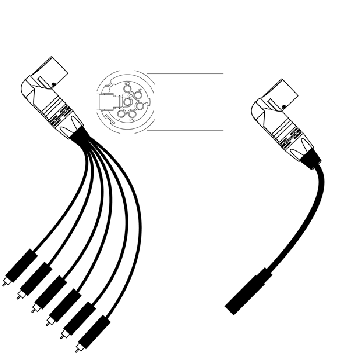
\includegraphics[width=70mm]{img-20-eps-converted-to-crop.pdf}
\caption{(a) Multi-adapter. (b) Mono-adapter}
\label{Smallwood:img-20}
\end{figure}

\section{Evaluation and Future Work}

In the performance of electronic music, the question of amplification is, of
course, an inherent concern.  The ultimate choices that are made about
amplification have an obvious effect upon the resulting music.  Our use of
personal hemispherical speakers has proven to be ``life changing,'' dramatically
altering the way we compose, improvise, and perform. It's an amazing to be able
to walk in to a room, unpack, plug in, and start playing music with others
without the usual concerns about speakers, mixers, and the rest of it.  It's all
right there. The change of sonic focus from a room-enclosing mass to a personal
resonator  has proven to be a fascinating place to work.  This is not to say that
we have created a ``better'' or more effective situation; rather, it simply
illustrates that we have found ourselves in a new place, which is always
exciting.  We hope to continue to find new ways of making sound with this
powerful resource, including some future outdoor, zero-carbon performances via
batteries and solar power.

\begin{acknowledgement}
Our most recent work has been supported by a John D. and Catherine T. MacArthur
Foundation Digital Media and Learning grant.
\end{acknowledgement}


\section*{Author Commentary: The Hemispherical Speaker and Beyond}

\paragraph{Scott Smallwood}

It has been six years since the publication of our paper on the loudspeaker experiments that resulted in a series of hemispherical speakers for laptop performance.  In that time, there has been a frenzy of new laptop orchestras and ensembles, individual laptop performers, and installation artists who have made use of hemispherical speakers of their own design, or those designed and sold by others (for example, Stephan Moore's Isobel speakers.)\footnote{\url{http://isobelaudio.com/}}  Indeed, the volume of innovations that have multiplied with the laptop ensemble phenomenon deserves its own book \cite{Bukvic:2010,Hantrakul:2013,Hopson:2014}!

At the time we wrote this article, it was a bit unusual for NIME to publish a ``how to'' guide, and we debated a lot about the right approach to doing that.  For us, it seemed important to not only discuss the history and motivation of what we were trying to do with sonic display, but to allow for an example of a specific speaker to be shown in nitty-gritty detail, even to the point of making references to specific parts, drawings of shell design, etc.  This was partially because we were getting so many questions from others who were trying to do this on their own, often with limited budgets.  It was also because, well, we had so much fun doing it, and wanted to share the process.  Obviously this paper rode a wave of DIY Maker-oriented projects on the web,\footnote{i.e. \url{http://www.instructables.com/}} which is why we produced a web-based version of the article as well, with links to specific parts and better quality images.  In the web version, we separated the DIY guide from the historical overview as two separate pages.\footnote{
\url{http://music2.princeton.edu/delorean/} and \url{http://music2.princeton.edu/delorean/history.html}}


The problem, of course, with such a specific set of instructions is that parts change or become obsolete.  The paper was a bit more general, but the web version mentioned above has an actual part list, with links to those parts, prices, etc.  We have made no attempt, for example, to update the listing of parts in the reprint here or on the web, but the industrious can easily find replacements.  Furthermore, we like to think that the original has the same kind of charm factor as those ephemeral publications from days gone by, such as the original Forrest M. Mims ``Electronic Music Projects'' book sold by Radio Shack \cite{Mims:1977}.  Our solution was just one of many, and for us it was more important to encourage people's sense of creativity and imagination rather than prescribing a specific solution.  We felt that giving a history, and a detailed snapshot of our present triumph was the most important goal.  Many have made use of the information in the article to their own ends, resulting in a diversity of projects and alternative sonic display systems for performance.  In fact, upon preparing for this article, a simple google search found dozens of hemispherical and related speaker designs. 

Speaker design for NIME has also been enhanced generally in the past ten years by the rise of inexpensive low power amplifiers, as well as increased access to computer-aided design of enclosures through technologies such as 3D printing and laser cutting.  One of our primary goals in creating the Delorean was to eliminate the rack of amps. The so-called ``Class T'' amplifier, initially by Tripath Technology \cite{Santo:2009}, enabled us to embed amplification directly inside the speaker.  Stephan Moore's Isobel speakers also make use of this design enhancement, while utilizing the warmer sound of MDF enclosures.  In addition, the use of alternative forms of transducers are also on the rise \cite{Bowers:2014}, as well as the use of actuators and other mechanical devices to pluck, strike, and otherwise physically move things other than speaker cones \cite{Kapur:2011a}.

I still use my Delorean to this day---and it still sounds great. I also regularly use one of the Isobel baritone speakers which also sounds wonderful, particularly in the lower end.  And in many of my synthesizer/sound designs, I routinely think in a six-channel orientation, even if ultimately the sounds are not played through a hemispherical speaker.  But just having that as a possibility has changed the way I think about channelization and distribution of voices or parameters.  More importantly, I think this research has helped to encourage makers to rethink the loudspeaker and its role in electronic music and sound art.  The innovations in speaker design are dizzying, as are the ways in which people amplify themselves.  We've come a long way since the beginnings of this research, and it will only get better from here.


\section*{Expert Commentary: From Local to Idiomatic}

\paragraph{Garth Paine}

The often heard phrase ``don't forget the loudspeaker'' is an important tenet in the development of electronic music, predating even Pierre Schaeffer's early music concrete explorations. Indeed the acousmatic tradition which grew out of Schaeffer and Henry's work at GRM in Paris, saw the rise of several loudspeaker orchestras, shifting focus to the loudspeaker as instrument, utilizing a range of loudspeaker drivers for varying timbre and engaging in spatialization and diffusion practices that are three-dimensional, immersive, dynamic and often performed live.

The expansion of these practices to include realtime processing of acoustic instruments brought about interesting discussions by Simon Emmerson on the question of ``local / field'' \cite{Emmerson:1994}---the sound of an acoustic cello (local) for instance within the immense spatial diffusion of real-time electronic processing spread over multiple loudspeakers (field). The question of location and context in terms of the sonic image has therefore been prevalent in early electronic music practices and scholarship for a considerable period of time.

Aligned with the development of almost ubiquitous processing tools for the personal laptop, and with that the exploration of massed laptop performances in the form of a laptop orchestra – the contemplation of the laptop as instrument, brings the aforementioned considerations into a new context. It is this context that is addressed in the associated article about the development and construction of hemispherical loudspeakers at Princeton University.

Indeed the authors refer to an ``outside-in approach'' in relation to placing a sounding source in a multichannel sound field such as a multichannel PA, implying a sense of scale of vastness of the amplification system as compared to the intimacy of the individual performer. The authors also referred to a desire to ``reduce the sonic power of electronic musicians and to increase the spatial abilities of those voices,'' and a desire to find ways of working with ``many voices in space and time, and creating an ensemble in which ensemble space and location are reclaimed as important and individuals sonic concepts.'' This dilemma comes about of course because the chameleon child of the industrial revolution [the personal computer] has no immediate affordances typically associated with a musical instrument---i.e. no inherent excitation-sonification relationship associated with music making, observable by an audience as a valid performative action. Underlying the research that produced these spherical loudspeakers is a strong desire to address this disassociation of the act of music making [excitation] from the observable, sonic outcome.

There is also an underlying discourse of democratization---the independence of a performer and the identification of individual voices, characteristics associated with acoustic instruments---traditionally the gold standard of music making. To this extent it is slightly perplexing that the hemispherical loudspeakers diffuse signal over a 360$^{\circ}$ radius on the horizontal plane, a characteristic that doesn't belong to the majority of acoustic instruments. Certainly the string instruments, woodwind and brass have a restricted diffusion angle which can be characterized through the use of mutes and/or holding the bell out directly towards an audience for particular effect. In that light hemispherical designs outlined in the paper provide for multiple loudspeaker drivers within the enclosure to be individually addressable, making this approach to diffusion unique by allowing special effects to be created as part of the identity of the diffusion practice \cite{Trueman:2000}. The attractiveness of this technical sophistication may however be in conflict with the constraints associated with the singular point of diffusion that remains consistent and is identified with an individual performance. In many ways acoustic instruments successfully develop idiomatic literature and communities of performances as a direct result of those  constraints rather than their individualized flexibility.

This last point is central to much discussion about NIME, where even sophisticated commercial interfaces are often marketed on the basis of flexibility and individualism rather than with a clear and defined role within the designated constraints. Perhaps the age of idiomatic music composition has passed? but then how do we consider the role of the individual within the ensemble, one of the instigating objectives for the development of the hemisphere loudspeaker. If we are going to prioritize music making with minimal constraints, it may direct us towards a community bound not by similarity but by difference, and bound by the form of practice derived from the chameleon child of the Industrial revolution. Only time will tell. The open source approach taken in this article also implies such a change---the DIY Maker movement has since become a major force in multi-disciplinary practice.

